\documentclass[hyperref={pdfpagelabels=false}]{beamer}
\usepackage{lmodern}
\usepackage[utf8]{inputenc}
\usepackage{amssymb}
\usepackage{amsmath}
\usepackage{tikz}
\usepackage{tkz-euclide}
\usetikzlibrary{arrows,calc,intersections,shapes,backgrounds,shadows}
\usetheme{Berlin}
\definecolor{UniRed}{RGB}{255,0,0}
\definecolor{UniWhite}{RGB}{255,255,255}
\setbeamercolor{eecks} {bg=UniRed, fg=UniWhite}
\title{\textsc{RoboSoccer} Project Plan}  
\author[Hofbauer, Jiang, Meyer, Schmidt, Wirnshofer]{
  Markus~Hofbauer \and
  He~Jiang \and
  Kevin~Meyer \and
  Benedikt~Schmidt \and
  Florian~Wirnshofer
}
\institute
{
	Technische Universit\"at M\"unchen, Germany
}
\date{June 4, 2014}
\begin{document}
\begin{frame}
\titlepage
\end{frame} 


\begin{frame}
	\frametitle{Table of contents}
	\tableofcontents
\end{frame} 

\section{Einleitung} 
\begin{frame}
	\frametitle{Einleitung} 
\end{frame}

\section{Class diagram}
\begin{frame}
	\frametitle{Layers}
	\center
	%!tikz editor 1.0
%!tikz source begin
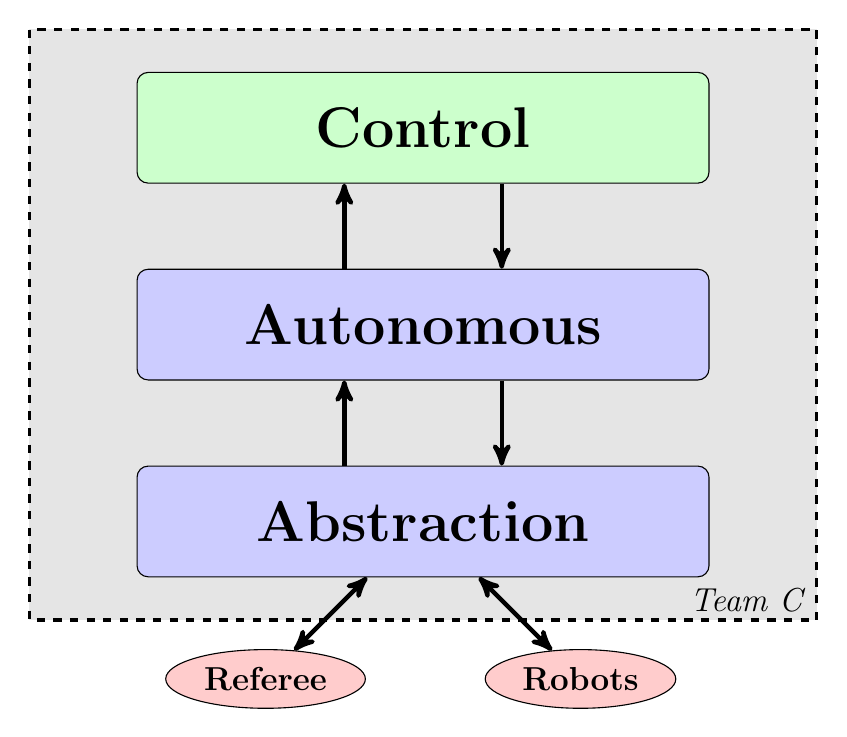
\begin{tikzpicture}
	
	\tikzstyle{block} = [
		rectangle, draw, fill=blue!20, 
		text width=20em, text centered, 
		rounded corners, minimum height=4em,
		node distance=2.5cm]
	
	\tikzstyle{block-active} = [
		rectangle, draw, fill=green!20, 
		text width=20em, text centered, 
		rounded corners, minimum height=4em,
		node distance=2.5cm]
		
	\tikzstyle{cloud} = [draw, ellipse,fill=red!20, node distance=2cm, minimum height=2em]
	
	\tikzstyle{line} = [draw, ->, >=stealth', ultra thick]
	\tikzstyle{dline} = [draw, <->, >=stealth', ultra thick]
	\tikzstyle{separator} = [draw, -, dashed, very thick]
		
    % Layers
	\node [block-active] (control) {\huge \textbf{Control}};
    \node [block, below of=control] (autonomous) {\huge \textbf{Autonomous}};
	\node [block, below of=autonomous] (abstraction) {\huge \textbf{Abstraction}};
	
	% Clouds
	\node [below of=abstraction, node distance=2cm] (babstraction) {} ;
	\node [cloud, right of=babstraction] (robots) {\large \textbf{Robots}};
	\node [cloud, left of=babstraction] (referee) {\large \textbf{Referee}};
    
	% Connections
	\path [line] ($(control.south) + (1,0)$) -- ($(autonomous.north) + (1,0)$);
	\path [line] ($(autonomous.north) + (-1,0)$) -- ($(control.south) + (-1,0)$);
	
	\path [line] ($(autonomous.south) + (1,0)$) -- ($(abstraction.north) + (1,0)$);
	\path [line] ($(abstraction.north) + (-1,0)$) -- ($(autonomous.south) + (-1,0)$);
	
	\path [dline] (referee) -- (abstraction);
	\path [dline] (robots) -- (abstraction);
	
	% Background Box
	\begin{pgfonlayer}{background}
		\draw [dashed, very thick, fill=black!10] ($(abstraction) +(5,-1.25)$) rectangle ($(control)+(-5,1.25)$);
		\draw ($(abstraction) +(5,-1)$) node [left] {\large \textit{Team C}};
	\end{pgfonlayer}
	
	
\end{tikzpicture}
%!tikz source end

\end{frame}

\begin{frame}
	\frametitle{Classes}
	\center
	%!tikz editor 1.0
%!tikz source begin
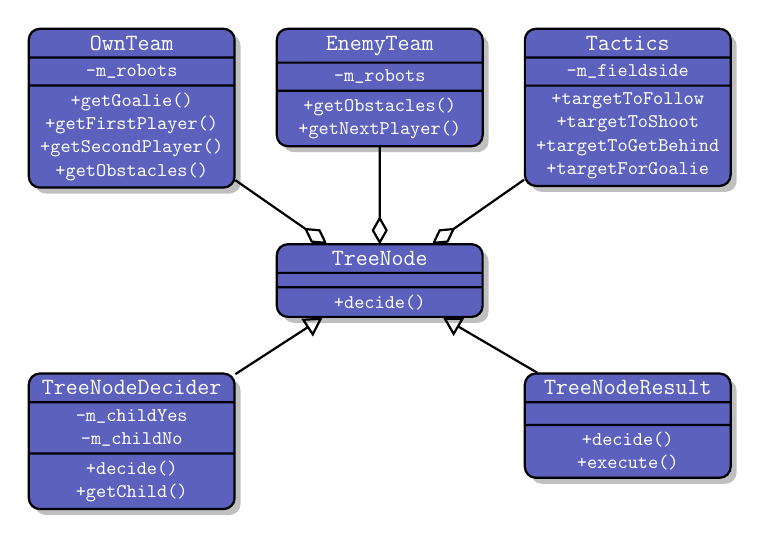
\begin{tikzpicture}[node distance=4.5cm, scale=0.7, transform shape]
	\font\btt=rm-lmtk10
	\definecolor{PresiBlue}{RGB}{50,57,171}
	
	\tikzstyle{class}=[
		rectangle, draw=black, rounded corners, rectangle split, rectangle split parts=3, 
		fill=PresiBlue!80, drop shadow, font=\tt,
        text centered, anchor=north, text=white, text width=3.5cm, thick]
		
	\tikzstyle{inheritance}=[draw, ->, >=open triangle 60, thick]
	\tikzstyle{property}=[draw, ->, >=open diamond, thick]
	\tikzstyle{line}=[-, thick]
   
   % Classes
      
	\node (treenode) [class]
	{
		{\large \texttt{\textbf{TreeNode}}}
		
		\nodepart{second}
		
		\nodepart{third}
		+decide()
	};
	
	\node (treenodedecider) [class, left =of treenode.south, anchor = north, yshift=-1cm]
	{
		{\large \texttt{\textbf{TreeNodeDecider}}}
		
		\nodepart{second}
		-m\char`_childYes\\
		-m\char`_childNo
		
		\nodepart{third}
		+decide()\\
		+getChild()
	} edge [inheritance] (treenode);
	
	\node (treenoderesult) [class, right =of treenode.south, anchor = north, yshift=-1cm]
	{
		{\large \texttt{\textbf{TreeNodeResult}}}
		\nodepart{third}
		+decide()\\
		+execute()		
	} edge [inheritance] (treenode);

	\node (ownteam) [class, left = of treenode.north, anchor = south, yshift=1cm]
	{
		{\large \texttt{\textbf{OwnTeam}}}
		
		\nodepart{second}
		-m\char`_robots
		
		\nodepart{third}
		+getGoalie()\\
		+getFirstPlayer()\\
		+getSecondPlayer()\\
		+getObstacles()
		
	} edge [property] (treenode);

	\node (enemyteam) [class, right = of ownteam.north, anchor = north]
	{
		{\large \texttt{\textbf{EnemyTeam}}}

		\nodepart{second}
		-m\char`_robots
		
		\nodepart{third}
		+getObstacles()\\
		+getNextPlayer()

	} edge [property] (treenode);

	\node (tactics) [class, right = of enemyteam.north, anchor = north]
	{
		{\large \texttt{\textbf{Tactics}}}
		
		\nodepart{second}
		-m\char`_fieldside
		
		\nodepart{third}
		+targetToFollow\\
		+targetToShoot\\
		+targetToGetBehind\\
		+targetForGoalie
	} edge [property] (treenode);


	% Connections
	
	
\end{tikzpicture}
%!tikz source end

\end{frame}

\section{State-Machine} 
\begin{frame}
	\frametitle{State-Machine} 	
\end{frame}

\section{Regelung} 
\begin{frame}
	\frametitle{Regelung}
\end{frame}

\section{Router} 
\begin{frame}
	\frametitle{Router} 
\end{frame}

\section{Gantt-Diagramm} 
\begin{frame}
	\frametitle{Gantt-Diagramm} 
\end{frame}

\end{document}

